Figure~\ref{fig:tvChannels} shows the power levels in the collection. Note that the X-axis is labeled with UHF TV channel numbers, each one $8$~MHz-wide and able to contain a maximum of four standard resolution or two high definition TV channels.

One of the tasks of the proposed algorithm~\cite{sanabriaCodeUSRP} is to assign a state (free or occupied) to each channel based on its power readings (in this case, thirty two readings per UHF TV channel). Each channel's state can be identified by looking at the right-hand side Y-axis in Figure~\ref{fig:tvChannels}.

A study performed by Domingo~\emph{et al.}~\cite{domingo2012white}, documented a spectrum sweep with a spectrum analyzer aimed at finding TV White Spaces at the same location as the testings in this work. The presented approach matched nearly 70\% of their observations, revealing 29 TV White Spaces against the 35 observed with the spectrum analyzer. This lower number is possibly due to narrow-band transmissions detected by the USRP.

\begin{figure}[htbp]
  \centering
  \includegraphics[width = 11cm, angle = -90]{sect3/figures/figure1_MACOM.eps}
  \caption{USRP-estimated TV White Spaces}
  \label{fig:tvChannels}
\end{figure}
